\documentclass[11pt,preprint, authoryear]{elsarticle}

\usepackage{lmodern}
%%%% My spacing
\usepackage{setspace}
\setstretch{1.2}
\DeclareMathSizes{12}{14}{10}{10}

% Wrap around which gives all figures included the [H] command, or places it "here". This can be tedious to code in Rmarkdown.
\usepackage{float}
\let\origfigure\figure
\let\endorigfigure\endfigure
\renewenvironment{figure}[1][2] {
    \expandafter\origfigure\expandafter[H]
} {
    \endorigfigure
}

\let\origtable\table
\let\endorigtable\endtable
\renewenvironment{table}[1][2] {
    \expandafter\origtable\expandafter[H]
} {
    \endorigtable
}


\usepackage{ifxetex,ifluatex}
\usepackage{fixltx2e} % provides \textsubscript
\ifnum 0\ifxetex 1\fi\ifluatex 1\fi=0 % if pdftex
  \usepackage[T1]{fontenc}
  \usepackage[utf8]{inputenc}
\else % if luatex or xelatex
  \ifxetex
    \usepackage{mathspec}
    \usepackage{xltxtra,xunicode}
  \else
    \usepackage{fontspec}
  \fi
  \defaultfontfeatures{Mapping=tex-text,Scale=MatchLowercase}
  \newcommand{\euro}{€}
\fi

\usepackage{amssymb, amsmath, amsthm, amsfonts}

\def\bibsection{\section*{References}} %%% Make "References" appear before bibliography


\usepackage[round]{natbib}

\usepackage{longtable}
\usepackage[margin=2.3cm,bottom=2cm,top=2.5cm, includefoot]{geometry}
\usepackage{fancyhdr}
\usepackage[bottom, hang, flushmargin]{footmisc}
\usepackage{graphicx}
\numberwithin{equation}{section}
\numberwithin{figure}{section}
\numberwithin{table}{section}
\setlength{\parindent}{0cm}
\setlength{\parskip}{1.3ex plus 0.5ex minus 0.3ex}
\usepackage{textcomp}
\renewcommand{\headrulewidth}{0.2pt}
\renewcommand{\footrulewidth}{0.3pt}

\usepackage{array}
\newcolumntype{x}[1]{>{\centering\arraybackslash\hspace{0pt}}p{#1}}

%%%%  Remove the "preprint submitted to" part. Don't worry about this either, it just looks better without it:
\journal{From Russia With No Love}

 \def\tightlist{} % This allows for subbullets!

\usepackage{hyperref}
\hypersetup{breaklinks=true,
            bookmarks=true,
            colorlinks=true,
            citecolor=blue,
            urlcolor=blue,
            linkcolor=blue,
            pdfborder={0 0 0}}


% The following packages allow huxtable to work:
\usepackage{siunitx}
\usepackage{multirow}
\usepackage{hhline}
\usepackage{calc}
\usepackage{tabularx}
\usepackage{booktabs}
\usepackage{caption}


\newenvironment{columns}[1][]{}{}

\newenvironment{column}[1]{\begin{minipage}{#1}\ignorespaces}{%
\end{minipage}
\ifhmode\unskip\fi
\aftergroup\useignorespacesandallpars}

\def\useignorespacesandallpars#1\ignorespaces\fi{%
#1\fi\ignorespacesandallpars}

\makeatletter
\def\ignorespacesandallpars{%
  \@ifnextchar\par
    {\expandafter\ignorespacesandallpars\@gobble}%
    {}%
}
\makeatother

\newenvironment{CSLReferences}[2]{%
}

\urlstyle{same}  % don't use monospace font for urls
\setlength{\parindent}{0pt}
\setlength{\parskip}{6pt plus 2pt minus 1pt}
\setlength{\emergencystretch}{3em}  % prevent overfull lines
\setcounter{secnumdepth}{5}

%%% Use protect on footnotes to avoid problems with footnotes in titles
\let\rmarkdownfootnote\footnote%
\def\footnote{\protect\rmarkdownfootnote}
\IfFileExists{upquote.sty}{\usepackage{upquote}}{}

%%% Include extra packages specified by user

%%% Hard setting column skips for reports - this ensures greater consistency and control over the length settings in the document.
%% page layout
%% paragraphs
\setlength{\baselineskip}{12pt plus 0pt minus 0pt}
\setlength{\parskip}{12pt plus 0pt minus 0pt}
\setlength{\parindent}{0pt plus 0pt minus 0pt}
%% floats
\setlength{\floatsep}{12pt plus 0 pt minus 0pt}
\setlength{\textfloatsep}{20pt plus 0pt minus 0pt}
\setlength{\intextsep}{14pt plus 0pt minus 0pt}
\setlength{\dbltextfloatsep}{20pt plus 0pt minus 0pt}
\setlength{\dblfloatsep}{14pt plus 0pt minus 0pt}
%% maths
\setlength{\abovedisplayskip}{12pt plus 0pt minus 0pt}
\setlength{\belowdisplayskip}{12pt plus 0pt minus 0pt}
%% lists
\setlength{\topsep}{10pt plus 0pt minus 0pt}
\setlength{\partopsep}{3pt plus 0pt minus 0pt}
\setlength{\itemsep}{5pt plus 0pt minus 0pt}
\setlength{\labelsep}{8mm plus 0mm minus 0mm}
\setlength{\parsep}{\the\parskip}
\setlength{\listparindent}{\the\parindent}
%% verbatim
\setlength{\fboxsep}{5pt plus 0pt minus 0pt}



\begin{document}



\begin{frontmatter}  %

\title{Russia-Ukraine Conflict}

% Set to FALSE if wanting to remove title (for submission)




\author[Add1]{Anna Mayer}
\ead{28776534@sun.ac.za}





\address[Add1]{Stellenbosch University}


\begin{abstract}
\small{
This report provides insights on aid allocation with regard to
Russia-Ukraine conflict and specifically analyses the ``commitment
gap'', showing which countries commited to more aid than they actually
allocated. A focus lies on EU member countries.
}
\end{abstract}

\vspace{1cm}


\begin{keyword}
\footnotesize{
Ukraine \sep Russia \sep Conflict \sep Aid \sep Commitment gap \\
\vspace{0.3cm}
}
\end{keyword}



\vspace{0.5cm}

\end{frontmatter}

\setcounter{footnote}{0}



%________________________
% Header and Footers
%%%%%%%%%%%%%%%%%%%%%%%%%%%%%%%%%
\pagestyle{fancy}
\chead{}
\rhead{}
\lfoot{}
\rfoot{\footnotesize Page \thepage}
\lhead{}
%\rfoot{\footnotesize Page \thepage } % "e.g. Page 2"
\cfoot{}

%\setlength\headheight{30pt}
%%%%%%%%%%%%%%%%%%%%%%%%%%%%%%%%%
%________________________

\headsep 35pt % So that header does not go over title




\hypertarget{introduction}{%
\section{\texorpdfstring{Introduction
\label{Introduction}}{Introduction }}\label{introduction}}

This report shows some rough insights into the Russia-Ukraine war, and
specifically analyses aid provided by countries in the EU. The report
focuses on whether the countries have kept their promises/ comitmments
in providing allocation. A focus lies on the commitment gap, which shows
whether the countries have pledged more aid than they have actually
provided.

\hypertarget{data}{%
\section{Data}\label{data}}

The data used is on aid commitments and allocation. In the analysis, I
focus on EU-member-countries and their commitments and actual
allocations.

\hypertarget{analysis}{%
\section{Analysis}\label{analysis}}

Let us first have a look at the relationship between GDP in 2021 and
total bilateral aid allocations. In general, one would expect a positive
relationship, which means that economically better off countries
allocate more.

\begin{figure}[H]

{\centering \includegraphics{Question3_files/figure-latex/Figure1-1} 

}

\caption{Who allocates Aid \label{Figure1}}\label{fig:Figure1}
\end{figure}

It seems that there is a general positive relationship between GDP in
2021 and total bilateral aid.

Nevertheless, one might be interested in whether the countries actually
allocated as much aid as they comitted initially.

\begin{figure}[H]

{\centering 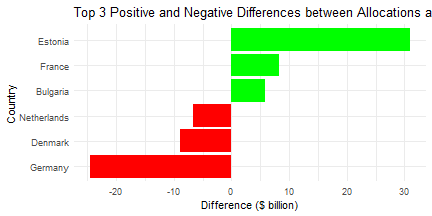
\includegraphics{Question3_files/figure-latex/Figure2-1} 

}

\caption{Commitment Gap \label{Figure2}}\label{fig:Figure2}
\end{figure}

The difference between allocations and commitment should be 0 if
countries allocated the same amount of money they actually committed to.
However, for some countries the difference is either greater and smaller
than 0. This graph shows the top 3 countries with greatest negative and
positive difference. Germany has the biggest committment gap. This means
that they committed to a much larger sum of total aid as compared to
their actuall aid allocation in \$billion. The same holds for Denmark
and the Netherlands. Estonia, France and Bulgaria actually allocated
more than they committed.

In a next step, this report checks whether there is a correlation
between Commitment Gap and GDP

\begin{figure}[H]

{\centering \includegraphics{Question3_files/figure-latex/Figure3-1} 

}

\caption{Commitment Gap and GDP \label{Figure3}}\label{fig:Figure3}
\end{figure}

Now, we can see that the relationship between the commitment gap and GDP
in 2021 is negative. This can be interpreted as that countries with
higher GDP have a larger commitment gap, which means that they actually
allocated less than they committed and the correlation seems relatively
strong. However, one has to acknowledge the large variation in the data,
especially with increasing GDP and that most data points are on the left
of the graph.

\hypertarget{conclusion}{%
\section{Conclusion}\label{conclusion}}

In conclusion, some countries have kept their promises and endeavored to
do enough to stem the tide of war. Although, economically better off
countries seem to allocate in general more (see \ref{Figure1}), when
looking at the difference between commitment and actual allocation, they
do not seem to keep there promieses (see \ref{Figure3}). Especially
countries with a higher GDP in 2021 (in \$billion), have not honored
their original pledges and have provided less funding, meaning that
there is a commitment gap for these countries.

\bibliography{Tex/ref}





\end{document}
